\section{Setting}
\label{sec:setting}

\subsection{Evaluation Metrics}
\label{subsec:evaluation_metrics}

The two main measurements for the performance of our new architecture are learning efficiency and transfer learning capability.
The learning efficiencies are measured in two different ways. First, the performance ILP(RL) is compared with exisitng RL algorithms in terms of
convergence rate, which is measured in terms of number of episodes that the agent needs to get to an optimal policy.
Second, the convergence of learning by ILASP is measured in terms of the number of hypothesis improvement devided by the total number of hypothesis improvement at episode 0.
The reason we are measuring it at only episode 0 is that empirically the agent learns the target hypothesis at episode 0 and there is no hypothesis refinement after episode 0.
This gives a normalised convergence rate of ILASP learning with the maximum 1.

\subsection{Benchmarks}
\label{subsec:benchmarks}

We use two existing RL methods as benchmarks: Q-learning and tile-coding.
Q-learning is widely used RL technique, and given the environments used for the experiments are discrete and deterministic, this method is sufficient enought for our experiment.

Another benchmark is tile coding, which is a type of linear function approximation techniques described in Chapter XX.
The reason for using an extra benchmark is that the comparision with q-learning might not be a fair comparision,
since ILP(RL) has one extra assumption: the agent knows surrounding information (whether there are walls in adjacent cells),
which is not a common assumption for Q-learning. Thus we incorporate the same surrounding information as features, and update the weights of each feature as a learning.
We compare the performance of ILP(RL) with these two methods.

\subsection{Parameters}
\begin{table}[!ht!b]
\centering
\begin{tabular}{lll}
\hline
Parameter            & ILP(RL)    & Benchmarks      \\ \hline
The number of episode& 100        & 100        \\
Time steps per episode& 250        & 250        \\
The number of experiments& 30       & 30       \\
% Discount rate        & 0,5       & 1.4e-2       \\
Alpha                & N/A       & 0.5       \\
Epsilon              & 0.1        & 0.1        \\
\end{tabular}
\caption{List of parameters used in the experiments}
\label{param}
\end{table}

All the matrices used in the experiments are summarised in Table \ref{param}.
Epsilon for ILP(RL) should be higher, since the agent follows the generated plan,
whereas benchmark algorithms update value function with the degree of alpha.
We conducted several experiments using different environments to highlight each aspect of the algorithm.

Since the performance of the agent is affected by the randomness of the exploration,
and ILP(RL) is highly dependent on how quickly the agent finds the goal,
each experiment is conducted 30 times and the perform is averaged across the experiments.
At each episode, we also measure the performance without exploration to see the pure optimal policy.

\section{Learning Evaluation}
\label{sec:learning_evaluation}

\subsection{Experiment Result 1}
\label{subsec:experiment_result_2}

\begin{figure}[!htb]
\centering
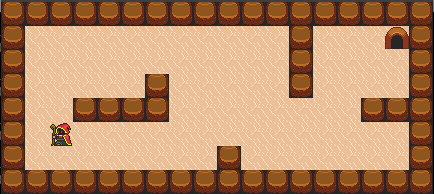
\includegraphics[width=0.5\textwidth]{./figures/experiment1}
\caption{Game environment for experiment 1}
\label{experiment1}
\end{figure}

The purpose of the first experiment is how the algorithm learns the model of the environment, or hypothesis in ILASP.
The environment are defined as a simple maze where the goal is located the right uppper corner as shown in Figure \ref{experiment1}.

The shortest path is taking the lower path instead of the upper one.

\begin{figure}[!htb]
\centering
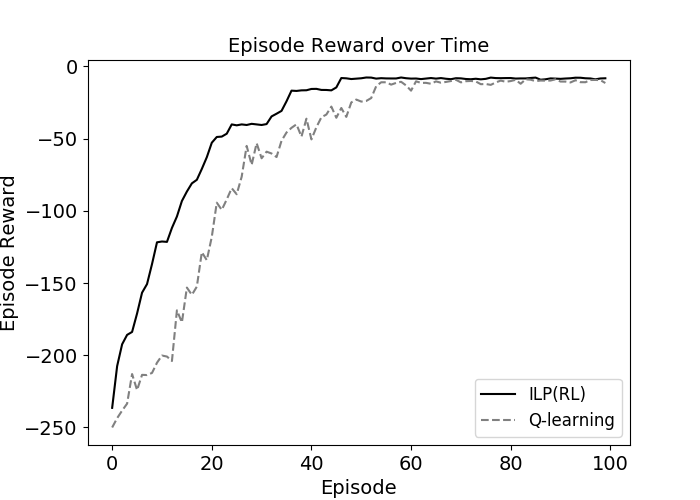
\includegraphics[width=1.0\textwidth]{./figures/experiment1_training}
\caption{Result of experiment 1 (learning curve)}
\label{experiment1_training}
\end{figure}
\begin{figure}[!htb]
\centering
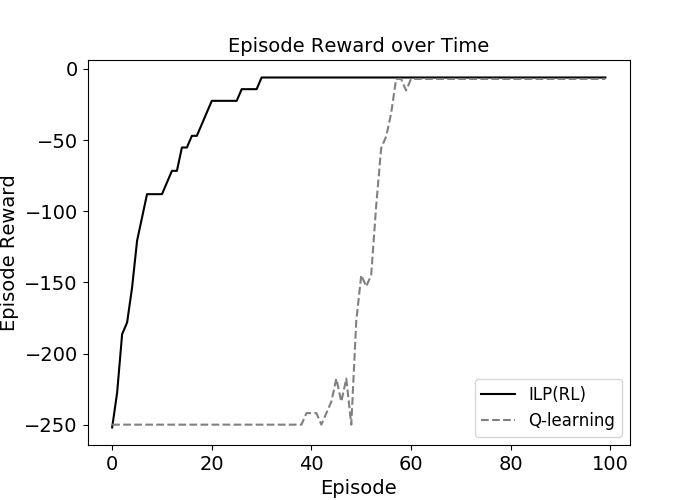
\includegraphics[width=1.0\textwidth]{./figures/experiment1_test}
\caption{Result of experiment 1 (performance)}
\label{experiment1_test}
\end{figure}

Figure \ref{experiment1_training} shows the traning performance between ILP(RL) and Q-learning.
The convergence rate of ILP(RL) is faster than Q-learning: ILP(RL) reaches the maximum reward between 40 and 50 episodes, whereas Q-learning reaches the same level at between 60 and 70 episodes.
This is because unlike Q-learning where the value function is updated with the rate of alpha, whereas ILP(RL) gradually builds the model of the environment and use the background knowledge to accurately plan.
This result is also consistent with the general notion that model-based learning (ILP(RL)) is more data-efficient than model-free learning (Q-learning).
The same trend is also shown in Figure \ref{experiment1_test}, where we measure only the performance of the policy without random exploration.

Overall this results shows that ILP(RL) converges to the optimal policy faster than benchmarks in a simple scenarios, achieving more data-efficient learning.

In addition to the data-efficient learning, what the agent has learnt with ILP(RL) is expressive.
Learnt hypotheses are shown in \ref{experiment1_hypothesis}, which is the rule of the game and easy to understand for human users.
Since the learnt hypothesis is a general concept, which can be used in a different environmet.
This transfer learning capability is also described in Experiement 3 and 4.

\begin{equation}
\begin{split}
&\textsf{state\_after(V1) :- adjacent(right, V0, V1), state\_before(V1), action(right), wall(V0).}\\
&\textsf{state\_after(V0) :- adjacent(right, V0, V1), state\_before(V0), action(left), wall(V1).}\\
&\textsf{state\_after(V1) :- adjacent(down, V0, V1), state\_before(V1), action(down), wall(V0).}\\
&\textsf{state\_after(V1) :- adjacent(up, V0, V1), state\_before(V1), action(up), wall(V0).}\\
&\textsf{state\_after(V0) :- adjacent(right, V0, V1), state\_before(V1), action(right), not wall(V0).}\\
&\textsf{state\_after(V0) :- adjacent(left, V0, V1), state\_before(V1), action(left), not wall(V0).}\\
&\textsf{state\_after(V0) :- adjacent(down, V0, V1), state\_before(V1), action(down), not wall(V0).}\\
&\textsf{state\_after(V0) :- adjacent(up, V0, V1), state\_before(V1), action(up), not wall(V0).}
\end{split}
\end{equation}
\label{experiment1_hypothesis}

In addition, we plot the learning convergence for ILASP at episode 0 in Figure \ref{experiment1_ilasp}, measured in terms of the number of hypothesis refinement to reach the final hypothesis as shown in \ref{experiment1_hypothesis}.
This shows that the agent quickly learns the hypothesis at the episode 0. The reason that the agent reaches the maximum reward at between 40 and 50 episodes, is mostly dependent on how quickly the agent finds the goal location,
which enables it to plan. Since our exploration strategy is expilon random choice, there is a promissing that a better exploration strategy further accelerates the learning process.

\begin{figure}[!htb]
\centering
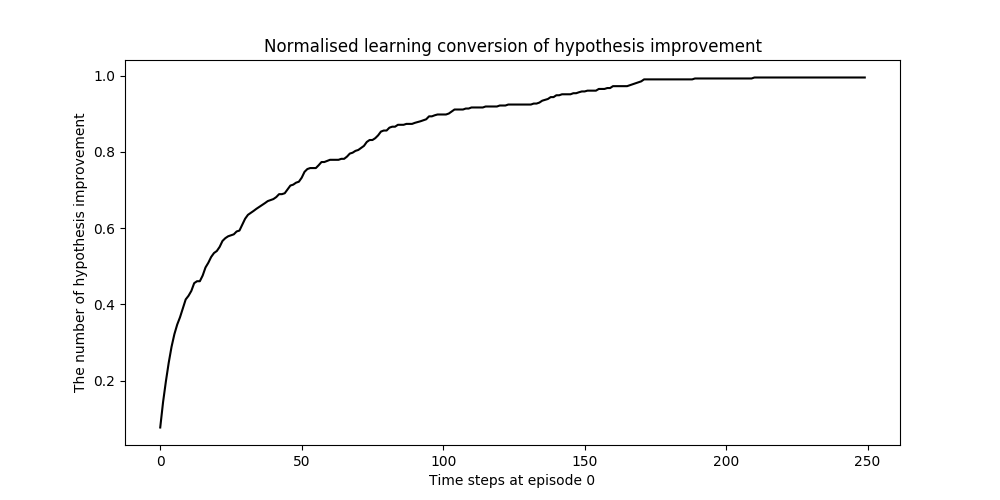
\includegraphics[width=1.0\textwidth]{./figures/experiment1_ilasp}
\caption{Normalised learning convergence by ILASP for experiment 1}
\label{experiment1_ilasp}
\end{figure}

\newpage
\subsection{Experiment Result 2}
\label{subsec:experiment_result_2}
% The game is designed such that

\begin{figure}[!htb]
\centering
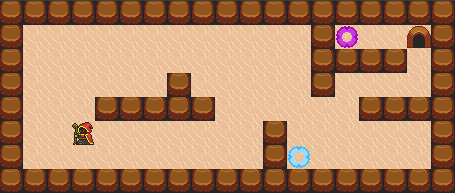
\includegraphics[width=0.5\textwidth]{./figures/experiment3}
\caption{Game environment for experiment 2}
\label{experiment3}
\end{figure}

Experiment 2 was conducted to see if the agent find a optimal path of using a teleport. In the environment shown in Figure \ref{experiment3},
there are two ways to reach the goal: using a normal path to get the goal located on the top right corner, or using a telport.
The environment is designed such that using a teleport is a shorter path and therefore gives higher total reward.
Compared to Experiment 1, two extra search spaces and concepts are added as follow:
\begin{equation*}
\begin{split}
&\textsf{\#modeb(1, link\_start(var(cell)), (positive)).}\\
&\textsf{\#modeb(1, link\_dest(var(cell)), (positive)).}
\end{split}
\end{equation*}

Where teleport links are added to the environment. The teleport link is one-way: link\_start takes the agent to link\_dest, but link\_dest does not take the agent back to link\_start.
The allows ILASP to learn additional hypothesis.
The full learning task for this experiment is in Appendix XX.

Once the agent steps onto a state where link\_start is located, it gets two positive experiences.
In this game environment, the agent moves two cells in one time step instead of one cell per time step.

Also link\_start and link\_dest need to be stored in background knowledge rather than as contex examples,
because ILASP needs to learn different hypothesis for link and non-link case.
link locations need to be available for all positive examples so that ILASP correctly learn non-link, which is shown in Figure XX below.

\begin{figure}[!htb]
\centering
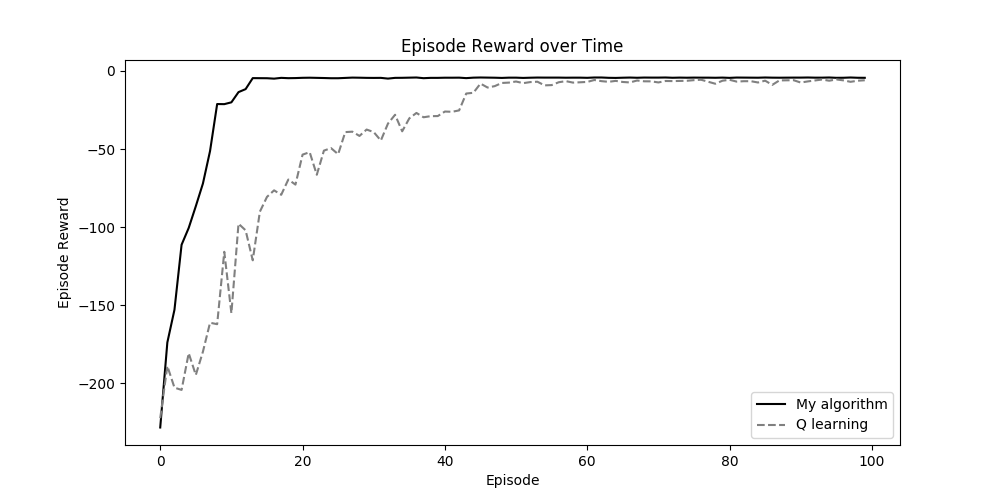
\includegraphics[width=1.0\textwidth]{./figures/experiment3_training}
\caption{Result of experiment 2 (learning curve)}
\label{experiment3_training}
\end{figure}

The training performance shown in XX, which converges faster than XX.

\begin{figure}[!htb]
\centering
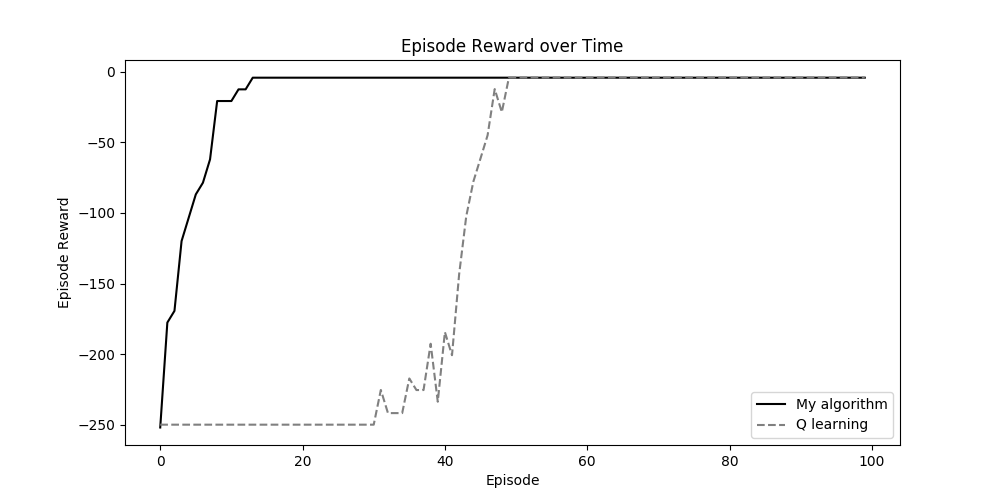
\includegraphics[width=1.0\textwidth]{./figures/experiment3_test}
\caption{Result of experiment 2 (performance)}
\label{experiment3_test}
\end{figure}

\begin{equation}
\begin{split}
&\textsf{state\_after(V1) :- link\_dest(V1).}\\
&\textsf{state\_after(V0) :- link\_dest(V0), state\_before(V0), action(right).}\\
&\textsf{state\_after(V1) :- adjacent(left, V0, V1), state\_before(V0), action(right), not wall(V1).}\\
&\textsf{state\_after(V0) :- adjacent(left, V0, V1), state\_before(V1), action(left), not wall(V0).}\\
&\textsf{state\_after(V1) :- adjacent(up, V0, V1), state\_before(V0), action(down), not wall(V1).}\\
&\textsf{state\_after(V0) :- adjacent(up, V0, V1), state\_before(V1), action(up), not wall(V0).}\\
&\textsf{state\_after(V1) :- adjacent(left, V0, V1), state\_before(V1), action(left), wall(V0).}\\
&\textsf{state\_after(V1) :- adjacent(down, V0, V1), state\_before(V1), action(down), wall(V0).}\\
&\textsf{state\_after(V1) :- adjacent(up, V0, V1), state\_before(V1), action(up), wall(V0).}
\end{split}
\label{experiment2_ilasp_imcomplete}
\end{equation}

To highlight the learning the new concept of teleport link, Figure \ref{experiment2_ilasp_imcomplete} is an intermediate incomplete hypothesis learnt by ILASP.
These hypotheses are generated just after the agent steps onto the link. However, the first hypothesis says
when link\_dest is available state\_after is true. Since link\_dest is available in background knowledge rather than context,
when solving for answer sets to generate a plan, it generates incorrect state\_after at every time step.
However, as shown in Algorithms XX, these generated state\_after are all incorrect and therefore will be added to exclusions of the next positive examples.
These exclusions will later refines hypotheses and results in Figure \ref{experiment2_ilasp_complete}, the final complete hypotheses.

Learnt hypotheses are as follow:
\begin{equation}
\begin{split}
&\textsf{state\_after(V1) :- link\_start(V0), link\_dest(V1), state\_before(V0).}\\
&\textsf{state\_after(V0) :- link\_dest(V0), state\_before(V0), action(right).}\\
&\textsf{state\_after(V1) :- adjacent(left, V0, V1), state\_before(V0), action(right), not wall(V1).}\\
&\textsf{state\_after(V0) :- adjacent(left, V0, V1), state\_before(V1), action(left), not wall(V0).}\\
&\textsf{state\_after(V1) :- adjacent(up, V0, V1), state\_before(V0), action(down), not wall(V1).}\\
&\textsf{state\_after(V0) :- adjacent(up, V0, V1), state\_before(V1), action(up), not wall(V0).}\\
&\textsf{state\_after(V1) :- adjacent(left, V0, V1), state\_before(V1), action(left), wall(V0).}\\
&\textsf{state\_after(V1) :- adjacent(down, V0, V1), state\_before(V1), action(down), wall(V0).}\\
&\textsf{state\_after(V1) :- adjacent(up, V0, V1), state\_before(V1), action(up), wall(V0).}
\end{split}
\label{experiment2_ilasp_complete}
\end{equation}

Compared the Experiment 1, there are two new hypotheses due to the presence of the teleport links.
These learnt hypotheses are also applicables to an environment where there is no link, such as a game in experiment 1.
In this case, the first two hypotheses in Figure XX are never be used since the body predicates relating to link\_start(V0), link\_dest(V1) are never be satisfied.

\begin{figure}[!htb]
\centering
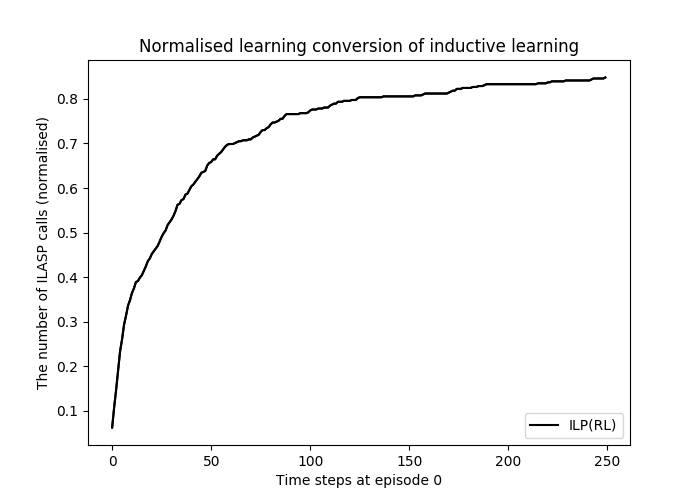
\includegraphics[width=1.0\textwidth]{./figures/experiment2_ilasp}
\caption{Normalised learning convergence by ILASP for experiment 2}
\label{experiment1_test}
\end{figure}

\newpage
\section{Transfer Learning Evaluation}
\label{sec:transfer_learning_evaluation}
\subsection{Experiment Result 3}

\begin{figure}[!htb]
\centerline{
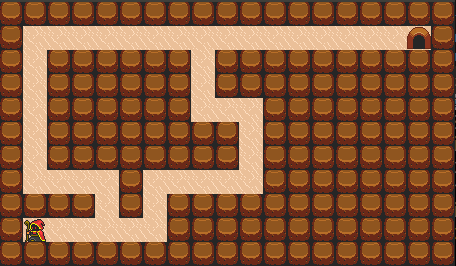
\includegraphics[width=0.5\textwidth]{./figures/experiment4_before}
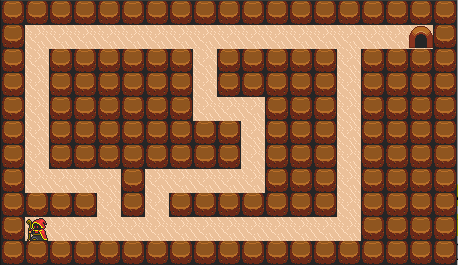
\includegraphics[width=0.5\textwidth]{./figures/experiment4_after}
}
\caption{Game environment for experiment 3: before (left) and after (right) transfer learning}
\label{experiment3}
\end{figure}

In Experiment 3, we investigated the potentials of transfer learning betweeen similar environments.
We trained the agent using the environment on the left in Figure \ref{experiment4}, and transfer the learnt hypothesis as well as positive examples to a new environment.
The learnt hypothesis is valid move of the game and a general concept that is applicable to any similar games. Positive examples are also transferred since
if there is a new concept that the agent needs to learn in a new environment, the agent needs to refine the hypothesis by running ILASP, thus the all the positice examples
are also transferred as well as hypotheses. Background knowledge are not transferred since these information are different in a new environment.
The agent starts with an empty background knowledge in the new environment and gradually collects them
as it explore the environment. The goal position is the same as in the first game and we assume that the transferred agent already knows the goal location, but the routes to the goal may be different.
While this is a limited transfer learning since the goal position is known in advance, this is still a useful transfer in cases where the rest of the environment changes.
In this experiment, we compare the two learning performance: one with transfer learning and one without it.
The result is shown in Figure \ref{experiment3_training} and \ref{experiment3_test}.

These are the hypotheses we are transferring to a new environment.
Since the complete hypothesis is already known to the agent, it can do planning from the beginning.

\begin{equation}
\begin{split}
 &\textsf{state\_after(V0) :- adjacent(right, V0, V1), state\_before(V1), action(right), not wall(V0).}\\
 &\textsf{state\_after(V0) :- adjacent(left, V0, V1), state\_before(V1), action(left), not wall(V0).}\\
 &\textsf{state\_after(V1) :- adjacent(down, V0, V1), state\_before(V0), action(up), not wall(V1).}\\
 &\textsf{state\_after(V0) :- adjacent(down, V0, V1), state\_before(V1), action(down), not wall(V0).}\\
 &\textsf{state\_after(V1) :- adjacent(right, V0, V1), state\_before(V1), action(right), wall(V0).}\\
 &\textsf{state\_after(V1) :- adjacent(left, V0, V1), state\_before(V1), action(left), wall(V0).}\\
 &\textsf{state\_after(V0) :- adjacent(up, V0, V1), state\_before(V0), action(down), wall(V1).}\\
 &\textsf{state\_after(V1) :- adjacent(up, V0, V1), state\_before(V1), action(up), wall(V0).}
\end{split}
\end{equation}

\begin{figure}[!htb]
\centering
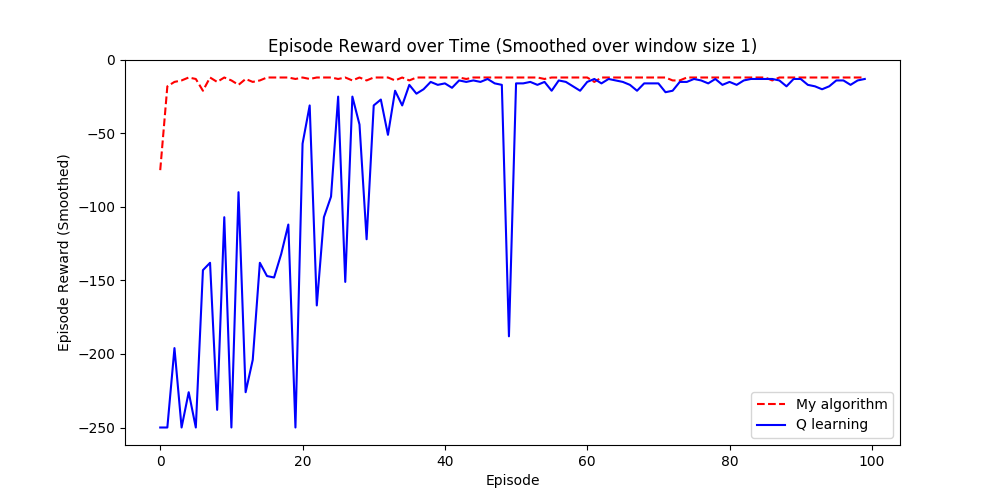
\includegraphics[width=1.0\textwidth]{./figures/experiment4_after_training}
\caption{Result of experiment 3 (learning curve)}
\label{experiment3_training}
\end{figure}

\begin{figure}[!htb]
\centering
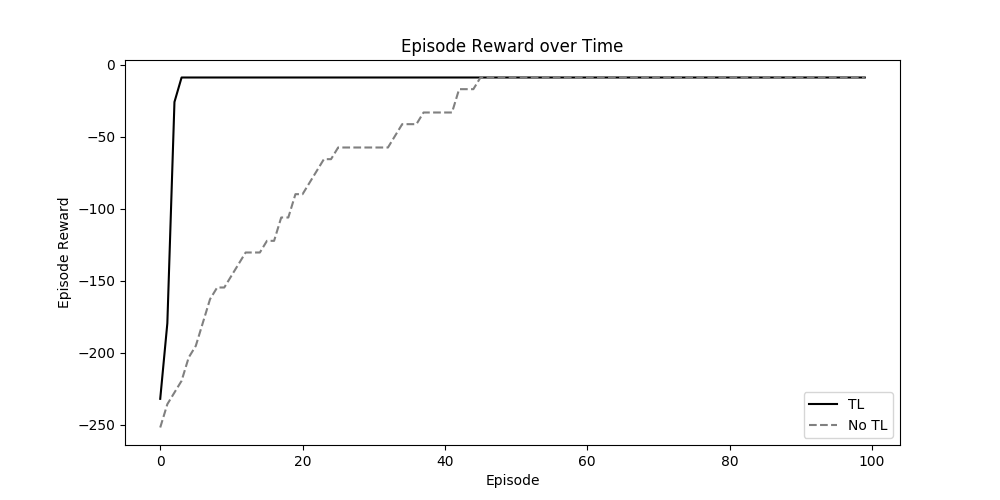
\includegraphics[width=1.0\textwidth]{./figures/experiment4_after_test}
\caption{Result of experiment 3 (performance)}
\label{experiment3_test}
\end{figure}

\subsection{Experiment Result 4}
\label{subsec:experiment_result_4}

\begin{figure}[!htb]
\centerline{
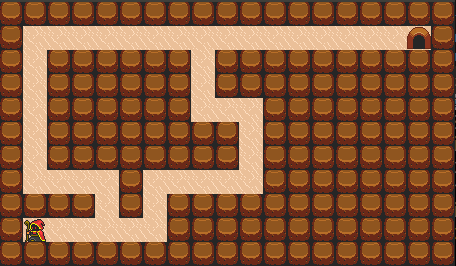
\includegraphics[width=0.5\textwidth]{./figures/experiment4_before}
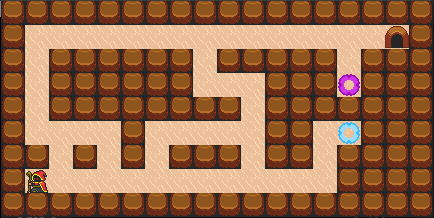
\includegraphics[width=0.5\textwidth]{./figures/experiment5_after}}
\caption{Game environment for experiment 4: before (left) and after (right) transfer learning}
\label{experiment5}
\end{figure}

Finally the hypothesis is transferred to a new environment where there is a new concept that did not exist in the first environment
and therefore the agent needs to learn it after the hypothesis is transferred.

\begin{figure}[!htb]
\centering
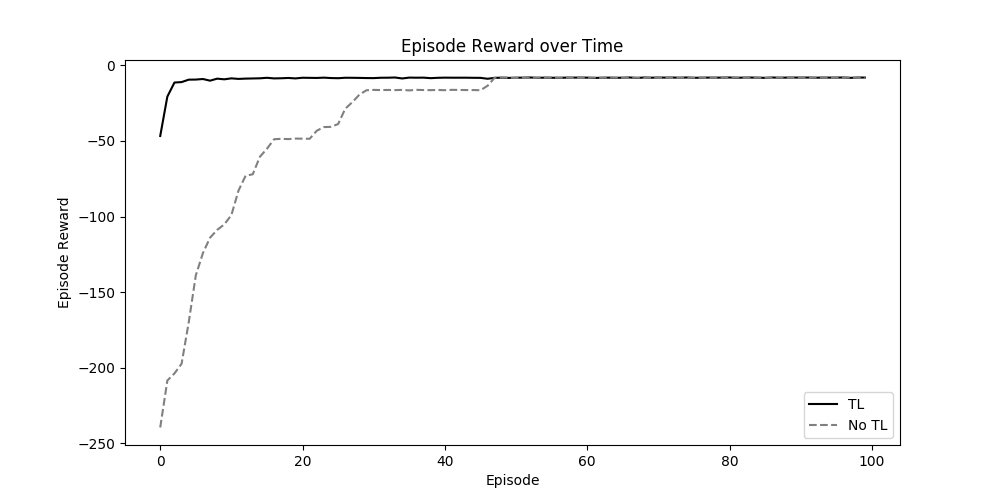
\includegraphics[width=1.0\textwidth]{./figures/experiment5_training}
\caption{Result of experiment 4 (learning curve)}
\label{experiment5_training}
\end{figure}

\begin{figure}[!htb]
\centering
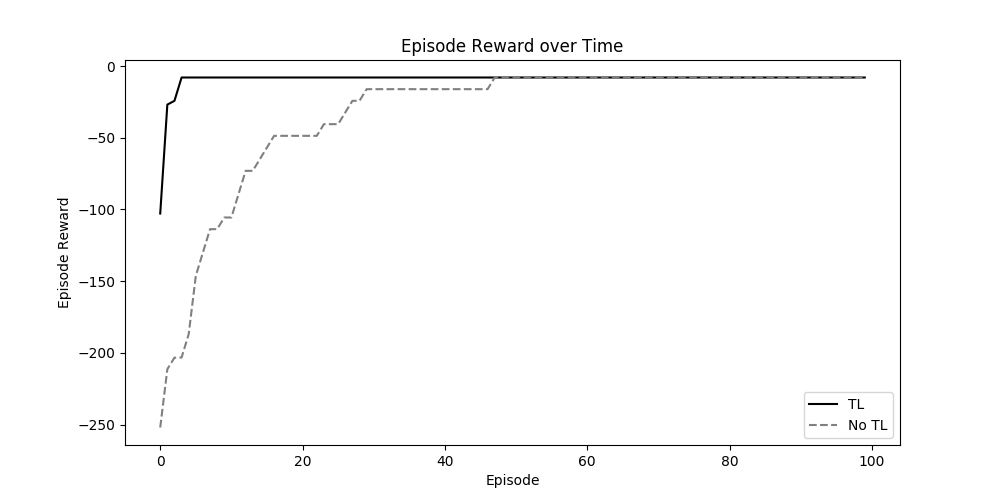
\includegraphics[width=1.0\textwidth]{./figures/experiment5_test}
\caption{Result of experiment 4 (performance)}
\label{experiment5_test}
\end{figure}

\begin{equation}
\begin{split}
&\textsf{state\_after(V1) :- link\_start(V0), link\_dest(V1), state\_before(V0).}\\
&\textsf{state\_after(V1) :- adjacent(left, V0, V1), state\_before(V0), action(right), not wall(V1).}\\
&\textsf{state\_after(V0) :- adjacent(left, V0, V1), state\_before(V1), action(left), not wall(V0).}\\
&\textsf{state\_after(V1) :- adjacent(up, V0, V1), state\_before(V0), action(down), not wall(V1).}\\
&\textsf{state\_after(V0) :- adjacent(up, V0, V1), state\_before(V1), action(up), not wall(V0).}\\
&\textsf{state\_after(V0) :- adjacent(left, V0, V1), state\_before(V0), action(right), wall(V1).}\\
&\textsf{state\_after(V1) :- adjacent(left, V0, V1), state\_before(V1), action(left), wall(V0).}\\
&\textsf{state\_after(V0) :- adjacent(up, V0, V1), state\_before(V0), action(down), wall(V1).}\\
&\textsf{state\_after(V1) :- adjacent(up, V0, V1), state\_before(V1), action(up), wall(V0).}
\end{split}
\label{experiment4_ilasp}
\end{equation}

\section{Strengths}
\label{strengths}

To my knowledge, this is the first attemp that inductive logic programming is incorporated into a reinforcement learning senario to facilitate learning process.
In simple environments, we show that the agent learns rule of the game faster than existing RL algorithms, learnt concepts is easy to understand for human users.
We also show that the learnt hypothesis is a general concept and can be applied to other environment to mitigate learning process.

The full hypotheses were learnt in the very early phase of learning and exploration phase. Thus with sufficient exploration, the model of the environment is correct
and therefore it is able to find the optimal policy/path. 

We show that ILP(RL) is able to solve a reduced MDP where the rewards are assumed to be associated with a sequence of actions planned as answer sets.
Although this is a limitated solution, there is a potential to expand it to solve full MDP as discussed in Further Research. 

TODO more details on the strength of the algorithm. 
Validity

\section{Limitations}

Although this is the first time and inductive logic programming is applied into reinforcement leaning and there are new interesting property for ILP(RL),
there are two major limitations with the current framework.

\subsection{Scalability}
The first limitation is scalability. As pointed in XXX or XXX,
ILP framework is known to be less scalable. The current framework is tested in a relatively simple environments, 
and proven to be work better than RL algorithsm in terms of the number of episodes that is needed to converge to an optimal policy.
However, learning in each episode is relatively slower than that of RL. 
This is shown in XXX, which shows average learnint time for ILASP. 

This limitation is theoretically discussed in XXX, where the complexity of deciding satisfiability is 
$\sum_{2}^{P}$-complete. Since there is no negative examples used in our current framework, the complexity is NP-complete.

Whereas Q-learning update value function in the same way whether there is a new concept such as teleport links.

Figure XXX shows traning times for Experiment 1 and 2.

ILASP learning time for Experiment 1 and 2. 

Unlike existing reinforcement learning,
out algorithm refines hypothesis at every time steps within the same episode.
Thus even though the efficiency in terms of the number of iteration is higher,
training time within each iteration tends to be lower.

\subsection{Flexibility}
While most of existing reinforcement learning works in different kinds of environment without pre-configuration, our algorithm
needs to define search space for learning hypothesis. As explained in the experiment 3, it was necessary to add two extra modeb before training.
Thus the algorithm may not be feasible in cases where these learning concepts were unknown or difficult to define. 
In addition, not only it needs search space, surrounding information is assumed to be known to the agent. 
While this assumption may be reasonable in many cases, this is not common in traditional reinforcement learning setting.

The current framework does not make use of rewards the agent collects and mainly uses the location of the goal for planning.
In some senarios, there may not be a termination state (goal) and instead there may be a different purpose to gain these rewards. 
Since the current implementation is dependent on finding the goal for planning rather than maximing total rewards, which is the common objective for most of RL algorithms,
the application of the current framework may be limited to particular types of problems.

Another question remains to how to extend the framework to more realistic senarios. RL works in more complex environments such as 3D or real physical environment, 
whereas the experiences of the agent in the current framework need to be expressed as ASP syntax, thus expressing continuous states rather than discrete states is challenging.